\documentclass[%
  unicode, % 文字コードの指定
  mathserif, %
  m, % vertical position of text: (t,m,b)
  % handout, % for printing slides
  aspectratio=169,
  12pt, %
  % compress,
  unknownkeysallowed
]{beamer}
%
% 各種設定用ファイルの読み込み:ここのファイル名は決め打ちにさせてください
%
  %
% パッケージの選択
%
\usepackage{luatexja}% 日本語に
\usepackage[haranoaji,deluxe]{luatexja-preset}% フォント指定
\renewcommand{\kanjifamilydefault}{\gtdefault}% 既定をゴシック体に
\usepackage{url}              % LaTeXの文章内にURLを貼りたいとき
\usepackage{hyperref}         % TeX 文書(DVI、PDF など)に HTML と同じハイパーリンク 機能を加えるためのマクロ
\usepackage{siunitx}          % LATEX で SI単位(国際単位系)を出力する
\usepackage{enumitem}         % リスト環境のレイアウトを制御
\usepackage{tikz}             % TeX 用の描画パッケージ
\usepackage{
    amsmath, % 環境
    amssymb, % 記号
    amsfonts % 特殊文字
}                             % amsmathの数式環境
\usetikzlibrary{positioning}     % ”positioning”ライブラリ
\usetikzlibrary{shapes.callouts} % 吹き出しの形を使うためにshapesライブラリを利用します
\usepackage[absolute,overlay]{textpos} % textposパッケージ
%\usepackage[colorgrid,gridunit=pt,texcoord]{eso-pic}
             % eso-picパッケージを使ってスライドの上からグリッドを表示、リリース時は消しておく
%\usepackage{layout}
             % layout パッケージもリリース時は消す
%
% デザインの選択
%     ここではテーマとしてmetropolisを読込
%
\usetheme[
    block=fill, % ブロックに背景をつける
    numbering=fraction % 合計ページ数を表示
]{metropolis}

%
% ここからはページの見え方の設定
%
% ページ番号
\setbeamerfont{frame numbering}{size=\large}
%
% CUD 配色の作成
% cf. http://bit.ly/2G99WCG
\definecolor{cud_blue}{rgb}{.109803922,.349019608,.682352941}
\definecolor{cud_green}{rgb}{.282352941,.639215686,.407843137}
\definecolor{cud_orange}{rgb}{.929411765,.564705882,.156862745}
\definecolor{cud_lightgray}{rgb}{.784313725,.784313725,.796078431}
%
% 基本色の変更
\setbeamercolor{normal text}{fg=cud_blue}
\setbeamercolor{example text}{fg=cud_green}
\setbeamercolor{alerted text}{fg=cud_orange}
%
% Navigation symbol は不要なので消す
\setbeamertemplate{navigation symbols}{}
%
% 見出しのスペースを消したい
\setbeamertemplate{frametitle}{
  \nointerlineskip
  \begin{beamercolorbox}[wd=\paperwidth,ht=2.25ex,dp=0.75ex]{frametitle} % htで直接指定
    \hspace*{1ex}\insertframetitle % 左margin + hspaceから始める
  \end{beamercolorbox}
}
%
% 図表番号を「図1」「表1」とかにする
\renewcommand{\figurename}{図}
\renewcommand{\tablename}{表}
\setbeamertemplate{caption}[numbered]
%
% 図とキャプションの間の余白
\setlength\abovecaptionskip{0pt}
%
% highlight マクロ tasusu.github.io/tikz.html から頂きました
\newcommand{\highlight}[2][yellow]{\tikz[baseline=(x.base)]{\node[rectangle,rounded corners,fill=#1!10](x){#2};}}
\newcommand{\highlightcap}[3][yellow]{\tikz[baseline=(x.base)]{\node[rectangle,rounded corners,fill=#1!10](x){#2} node[below of=x, color=#1]{#3};}}
%
%footer修正
\def\logoC{opencae-logo.png}
\def\logoD{kotohajime.png}
\makeatletter
\setbeamertemplate{footline}{
    \begin{columns}[totalwidth=160mm]
      \begin{column}{24.1mm}
        \includegraphics[width=24.1mm, height=5mm]{work/images/\logoC}
      \end{column}
      \begin{column}{104mm}
         {\scriptsize \color{cud_lightgray} \insertshortinstitute / \insertshortdate{}  (\insertshortauthor) }
      \end{column}
      \begin{column}{16mm}
         {\footnotesize \color{cud_orange} \rightline{ \insertframenumber{} / \inserttotalframenumber}}
      \end{column}
      \begin{column}{15mm}
        \includegraphics[width=15mm, height=5mm]{work/images/\logoD}
      \end{column}
    \end{columns}
}
   % 資料毎に変えない設定を読み込む
  % 表題の例
%     title     に主題
%     subtittle に副題を設定(省略可)
%
\title{圧力容器の応力値を手計算とCAEで比較した}
\subtitle{~ PrePoMaxは、やればできる子~}
%
% 日付/発表者設定の例
%     date      に発表日の日付
%     author    に発表者の名前
%     institute には本来は発表者の所属先ですが、下の例では発表会の名前とした
%     それぞれ左の角カッコ内が簡易表記で、表紙以外で使われ
%     右の波カッコ内が詳細表記で、表紙で使われる
%
\date[2-24-2024]{発表日:2024年2月24日}
\author[ichmy55]{発表者:ichmy55}
\institute[  25th Meeting/OpenCAE Local User Group@Kantou(str)]{報告:第25回オープンCAE勉強会@関東(構造など)}
  % 資料毎に変える設定を読み込む
%
% ここから、各章毎に分割したソースファイルを順番に読込
%
\begin{document}
  %
  \maketitle                    % 表紙の出力指示(省略してもよい)
  %\section{本ソフト/資料の目的} % セクション表紙の出力指示(省略してもよい)
  \begin{frame}{お品書き}
  \begin{enumerate}[label=\textbf{ \arabic*.},itemsep=1.3ex, leftmargin=1cm]
    \item 自己紹介
    \item 本日の例題
    \item 以前の計算結果と指摘
    \item 改めて解いてみた(PrePoMaxは、やればできる子)
    \item 結果の紹介
    \item まとめ
  \end{enumerate}
\end{frame}

  %\input{src/012-chapter1-2}
  %\input{src/013-chapter1-3}
  %\input{src/014-chapter1-4}
  %\input{src/015-chapter1-5}
  %%%
  \begin{frame}{4面体メッシュ切り(成功例)}
 
% 図の挿入
\begin{figure}[htbp]
\begin{center}
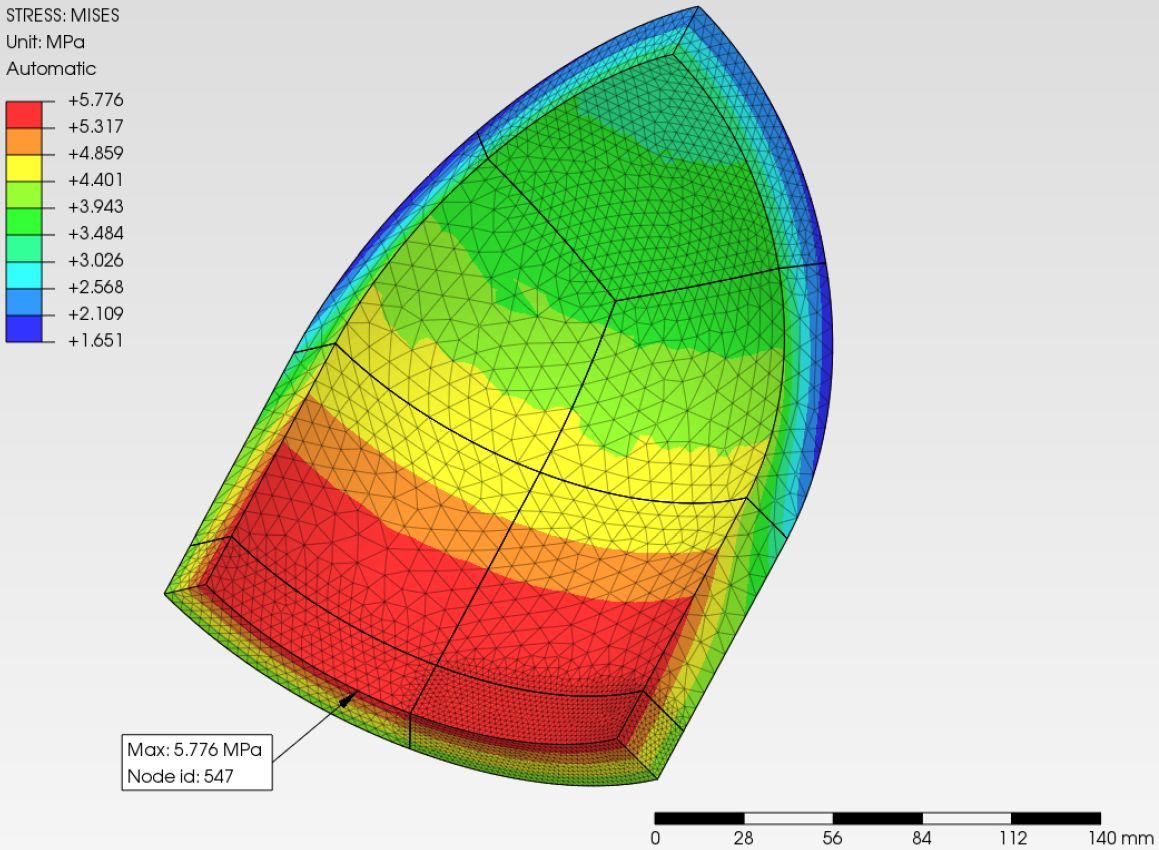
\includegraphics[keepaspectratio,scale=1.0]{work/images/fig01.jpg}
\caption{4面体メッシュ切り(成功例)}
\end{center}
\end{figure}
 
\end{frame}

  \begin{frame}{6面体メッシュ切り(成功例)}
 
% 図の挿入
\begin{figure}[htbp]
\begin{center}
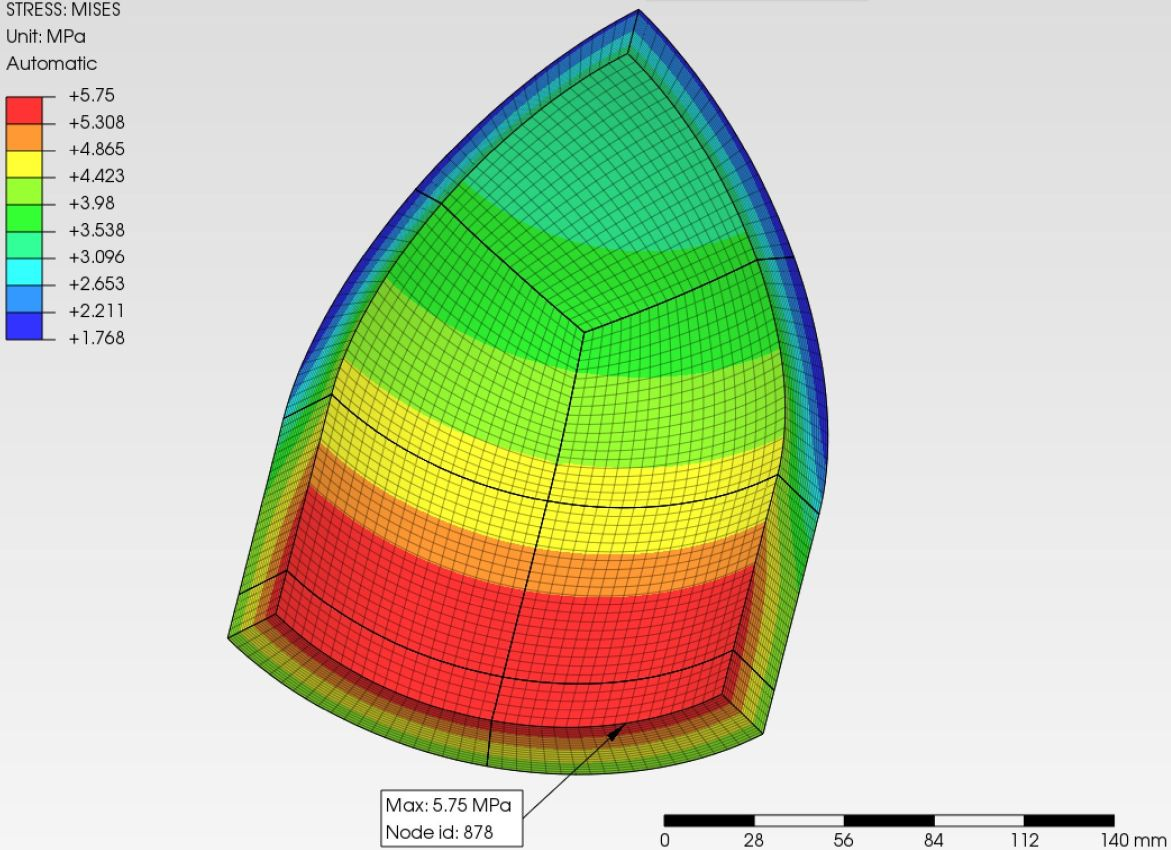
\includegraphics[keepaspectratio,scale=1.0]{work/images/fig02.jpg}
\caption{6面体メッシュ切り(成功例)}
\end{center}
\end{figure}
 
\end{frame}

  \begin{frame}{6面体メッシュ切り(失敗例)}
 
% 図の挿入
\begin{figure}[htbp]
\begin{center}
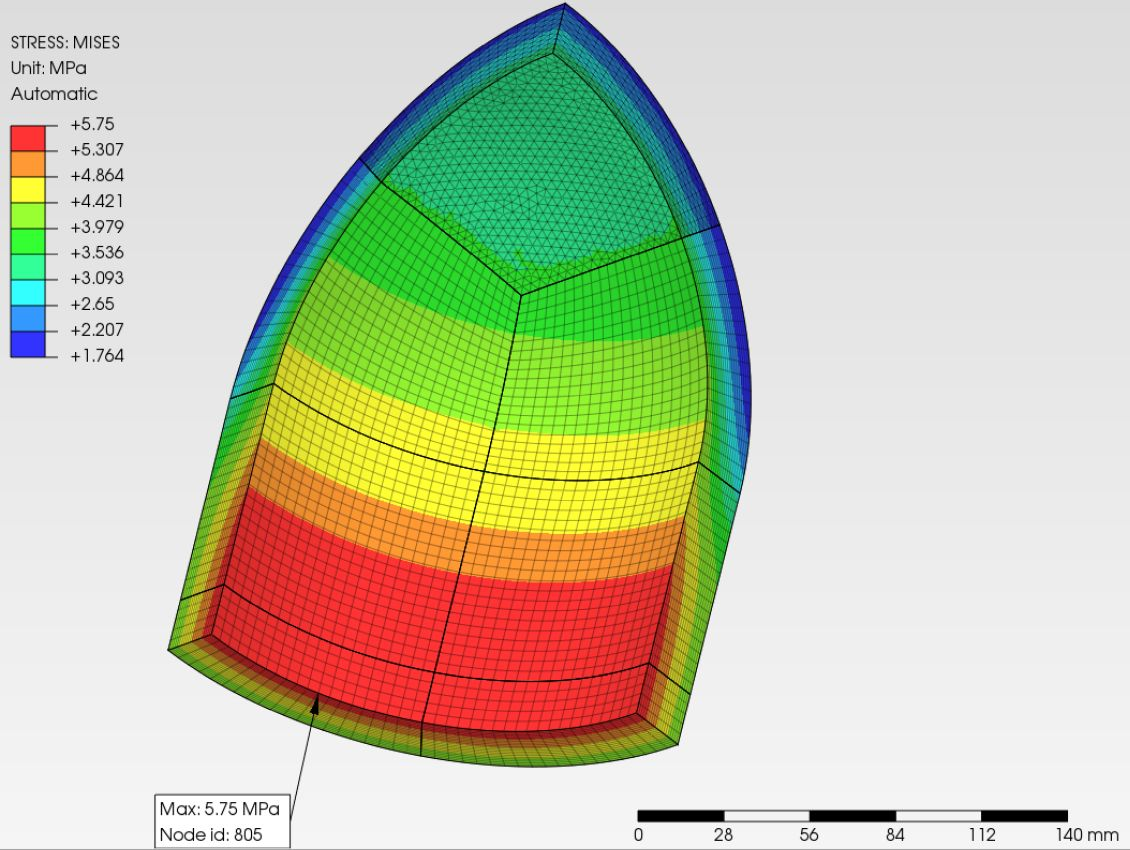
\includegraphics[keepaspectratio,scale=1.0]{work/images/fig03.jpg}
\caption{6面体メッシュ切り(失敗例)}
\end{center}
\end{figure}
\end{frame}

  %%%
  \begin{frame}{参考文献}
  \begin{enumerate}[label=\textbf{[\arabic*]},itemsep=1ex, leftmargin=1mm]
      \item オープンCAE勉強会@関西.“オープンCAE Wanted@関西”.\\
          {\footnotesize \urlstyle{same}
          \url{https://scrapbox.io/opencae-wanted/第76回:圧力容器の応力値を手計算とCAEで比較した}} \\
          (参照 2024-02-23)
     % \item @Sagittarius_Chiron.“PrePoMax使用法解説ー3.0 複合材”.Qiita.\\
      \item @Sagittarius\_Chiron.“PrePoMax使用法解説ー3.0 複合材”.Qiita.\\
          {\footnotesize \urlstyle{same}
          \url{https://qiita.com/Sagittarius_Chiron/items/6a885ea8ee8f35c7a89c}} \\
          (参照 2024-02-23)
  \end{enumerate}
\end{frame}

  \begin{frame}[noframenumbering]{}
	ご清聴、ありがとうございました

  % この場合は (150pt, 150pt) の位置に 0.6\linewidth の幅のブロックができる.
  \begin{textblock*}{0.7\linewidth}(100pt,180pt)
    % TiKZを使った図形の描画
    \begin{tikzpicture}
        \node[rectangle,fill=cyan!10,text width=320pt,text centered,rounded corners,minimum height=50pt,align=left]
           { \scriptsize (このスライドのTexソースは \\
             \urlstyle{same}
             \url{https://github.com/ichmy55/opencae-slides/tree/main/src/opencae-kantou-s-025} \\
             にあります。よければご参照ください
           };
    \end{tikzpicture}
  \end{textblock*}
\end{frame}

\end{document}
